\section{Simulación de la demanda de alumnos}

La demanda del número de alumnos para el siguiente semestre la hicimos por materia y por hora. Para poder hacer la simulación lo primero que hicimos fue acomodar la información que teníamos por semestres y por hora. El procedimiento que seguimos es el siguiente:

\begin{enumerate}
\item Definir el semestre del cual se quiere obtener la simulación.

\item Definir el número de semestres que se quieren como ventana de información.

\item Tomar una submatriz de \textit{m\_grande\_total} con la información de una materia para los semestres en la ventana de información.

\item Para cada semestre dentro de la ventana de información se suma el número de alumnos en cada hora.

\item Se obtiene una matriz de $15 \times k$ ($k$ es el número de semestres en la ventana) como la que se puede ver en la figura \ref{matAl_corregidos}.
\end{enumerate}

\begin{figure}[H]
\centering
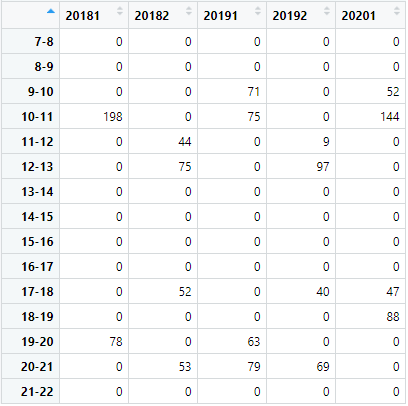
\includegraphics[scale = 0.8]{mat_alumnos_corregidos_EstadisticaIII} %width=\textwidth
\caption{\textit{Ejemplo de matriz con alumnos corregidos}}\label{matAl_corregidos}
\end{figure}

Con el procedimiento descrito pudimos generar vectores por hora y aplicar la función \verb@hw()@ en \textit{R} para obtener la demanda de alumnos esperados para el siguiente semestre. En la figura \ref{vec_alum_sim} vemos el vector con la demanda de alumnos simulados para el semestre 2020-2 de la materia \textit{Estadística III}.

Notamos que el valor de la demanda de alumnos es cero cuando en todos los semestres de alguna hora no hay datos. En el ejemplo, es el caso de las 7hrs, 8hrs, 13hrs, 14hrs, 15hrs, 16hrs y 21hrs.

Observando los datos de las 10hrs. vemos que en los semestres pares no hay alumnos, por lo que en la simulación se obtiene únicamente un alumno. Si vemos los datos de las 17hrs vemos que de los 5 semestres en la ventana se tienen alumnos en los semestres pares y en un semestre impar, el número de alumnos simulados para esa hora son 31 alumnos.

Con estos ejemplos podemos ver de manera tangible que el modelo si respeta la estacionalidad semestral que tienen los datos.

\begin{figure}[H]
\centering
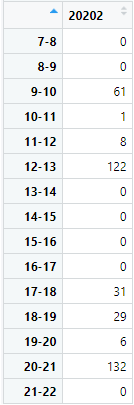
\includegraphics[scale = 0.8]{vec_alum_sim_EstadisticaIII} %width=\textwidth
\caption{\textit{Ejemplo de vector con demanda simulada para el 2020-2}}\label{vec_alum_sim}
\end{figure}

Obtuvimos vectores con la demanda simulada para cada una de las materias y formamos una matriz de $15 \times 333$. En la figura \ref{matDemandaAlum} podemos ver un ejemplo de cómo se ve la matriz formada.

Analicemos 2 pares de grupos, primero veamos la segunda y la quinta columna, que corresponden a las materias de \textit{Álgebra Superior II} y \textit{Geometría Analítica I}, respectivamente. Ambas son materias obligatorias para Actuaría, Matemáticas y Matemáticas Aplicadas. La primera corresponde a semestres pares y la segunda a semestres pares. Notamos que para \textit{Geometría Analítica I}, se tienen alumnos prácticamente en cada hora, pero el número no es muy grande, a diferencia de los alumnos simulados para \textit{Álgebra Superior II}, en donde hay varias horas con cero alumnos simulados pero hay dos grandes cantidades, una a las 9hrs con 832 alumnos y la otra a las 18hrs con 224 alumnos. Con esta comparación podemos ejemplificar la diferencia entre una materia que corresponde a semestres pares con una de semestres impares.

Ahora analicemos las columnas 4 y 8, correspondientes a las materias de \textit{Seminario de Topología A} y \textit{Probabilidad II}. La primera es una materia optativa para Matemáticas y la segunda es una materia obligatoria para Actuaría, correspondiente a semestres pares y optativa para Ciencias de la Computación, Matemáticas y Matemáticas Aplicadas. El número total de alumnos simulados para \textit{Seminario de Topología A} es menor a 20, en cambio para \textit{Probabilidad II} se tiene una gran cantidad de alumnos a las 8hrs, 9hrs y 10hrs. Considerando los valores que se tienen en el turno vespertino para \textit{Probabilidad II}, notamos que a las 19hrs también hay una gran cantidad de alumnos. Con esta comparación podemos ejemplificar la diferencia entre una materia obligatoria y una optativa, así como la diferencia entre el turno matutino y vespertino.


\begin{figure}[H]
\centering
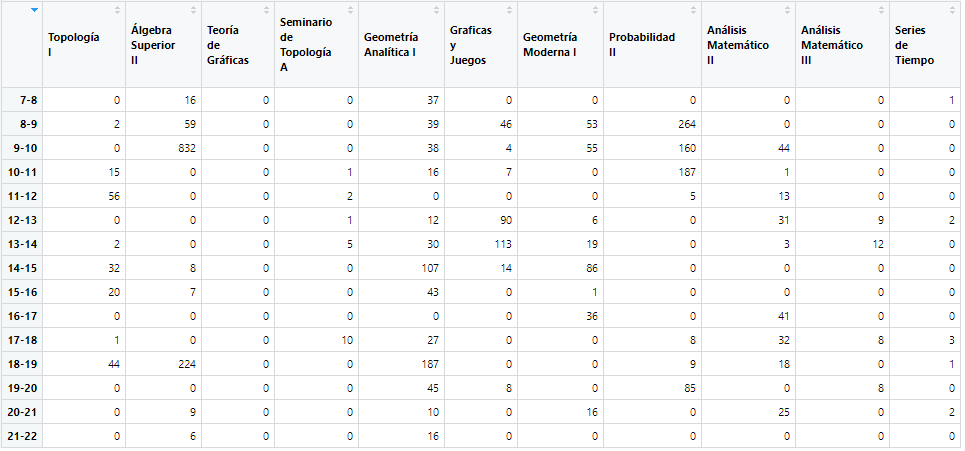
\includegraphics[scale = 0.7]{mat_demanda_alumnos} %width=\textwidth
\caption{\textit{Ejemplo de matriz con demanda simulada para el 2020-2}}\label{matDemandaAlum}
\end{figure}
